\chapter{Financial Plan}\label{ch:finance}

\section{Break-even logic}\label{sec:breakeven}
Following the logic of Gustafsson et al.~\cite{gustafsson2021}, a fit tool pays for itself when it costs the retailer less per order than the fit-related return cost it avoids. Our version of that logic is
\begin{equation}\label{eq:breakeven}
  c_{\mathrm{be}} = \rho \times r \times \varphi \times c,
\end{equation}
where $\rho$ is the relative reduction of fit-related returns, $r$ the return rate of online apparel orders, $\varphi$ the fit-related share of returns and $c$ the cost of one return. We use $r=24.4\%$ from a US survey~\cite{coresight2023}, $c=\$6.80$ (17\% of an assumed prime cost of \usd{40}), $\varphi=40\%$ and $\rho=15\%$, the last three \assumed{assumed} inputs. The 17\% comes from one footwear retailer, where it is the return cost per pair sold, not per return~\cite{gustafsson2021}. Because only a share of pairs is returned, the cost of one return in that study is higher than 17\% of prime cost. Using \usd{6.80} per return is therefore a conservative lower bound: a higher cost per return would raise the retailer's saving. Prime cost is also our own assumption of 50\% of the order value, not the retailer's purchase price as in the source. These inputs give $c_{\mathrm{be}}=\derived{\usd{0.0996}}$ per order. The blended price of \usd{0.036} (about \ils{0.13}) is 36\% of that value.

The reduction $\rho=15\%$ applies to the whole shop. Only 25\% of orders include a scan (an \assumed{assumed} share), so a 15\% shop-wide reduction means about a 60\% reduction of fit-related returns among scanned orders, if the tool acts only on those orders. That is above the 40\% low scenario of Gustafsson et al.\ and cannot be called modest. The pilot has to show it. The model also bills every order of a client, not only scanned orders. If billing covered scanned orders only, revenue would fall in proportion, and we flag that the billing base must be fixed in the contract.

\section{Five-year projection}\label{sec:projection}
Figure~\ref{fig:f5} shows the model output. Revenue grows from \usd{10,000} in year 1 to \derived{\usd{782,000}} in year 5, of which Israeli subscriptions are only \usd{54,000}. The operating result is negative in every year: \usd{-272,000}, \usd{-347,750}, \usd{-423,500}, \usd{-771,375} and \usd{-517,750}. The cumulative deficit is \derived{\usd{2,332,375}} at the end of year 5. There is no operating profit within the five-year horizon. The funding ask is the cumulative deficit plus a 20\% buffer (\assumed{assumed}), which is \derived{\usd{2,798,850}}, or about \usd{2.8} million. It funds the plan through year 5 only.

Year 6 is an extrapolation outside the model, not a result. A hand calculation shows that run-rate break-even needs about 37 European paying clients, and that the plan could reach that number in year 6, but only if the team stays at 12, no client leaves and payroll and pilot costs are the only costs. None of these holds by construction. The model has no churn, and it leaves out cost lines a real company would carry, among them marketing and customer acquisition, cloud base cost, legal and compliance review, travel and general administration. We list them as a limitation rather than add numbers we cannot source. The scan cost of \usd{0.03} and the person-year cost of \usd{90,000} are assumptions with no benchmark behind them.

Three limits are stated openly. First, Israel's addressable fee pool is only about \usd{198,000} a year (Chapter~\ref{ch:market}), so Europe carries the revenue. Of the \usd{782,000} in year 5, \usd{648,000} comes from one chain of assumptions: 18 European clients, each averaging one million orders a year, each paying for its whole first year. The one million orders per client has no source. Billing for the whole first year is a simplification, since a nine-month sales cycle and a pilot would delay the first invoice. Second, the 50\% conversion of pilots to paying clients is assumed, and the Israeli path converts at only about 35\% (Chapter~\ref{ch:gtm}). Third, Table~\ref{tab:company-sens} shows how the company's result changes when conversion, orders per client and the year of Europe entry change, so a reader can see that the plan does not rest on one case.

\begin{figure}[tbp]
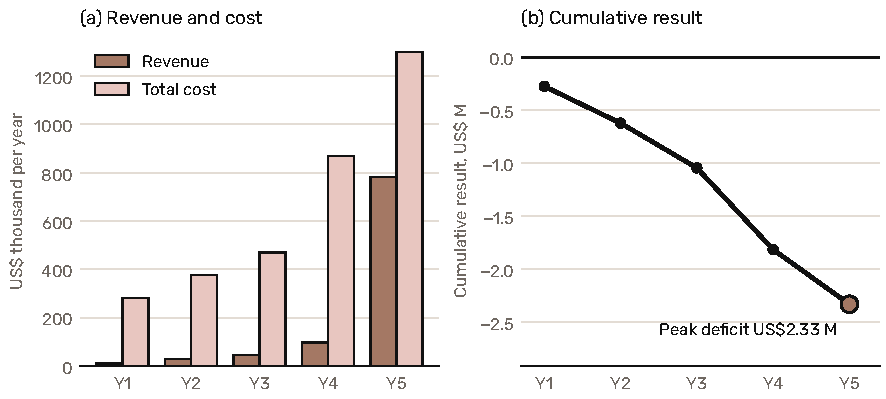
\includegraphics[width=\textwidth]{figures/f5-projection.pdf}
\caption{Five-year projection and cumulative result (model output; no operating profit in the horizon)}\label{fig:f5}
\end{figure}

\begin{table}[tbp]
\caption{Company-level sensitivity (model output; the rows are defined in the text)}\label{tab:company-sens}
% Company-level sensitivity (python/company_sensitivity.py). All amounts US$ thousand. Caption and label tab:company-sens: qa-se.
\ctnumcols{5}
\begin{tabularx}{\textwidth}{WVVVVV}
\toprule
\ctheaderrow\cthead{Scenario (US\$ thousand)} & \cthead{Y5 revenue} & \cthead{Y5 result} & \cthead{Peak deficit} & \cthead{Ask} & \cthead{Break-even clients}\\
\midrule
Base case & 458 & $-$998 & 3\,249 & 3\,899 & 44\\
Pilot-to-paying 35\% & 345 & $-$1\,088 & 3\,362 & 4\,035 & 44\\
Orders 500\,k & 296 & $-$1\,127 & 3\,377 & 4\,053 & 88\\
Low-touch 250\,k & 276 & $-$1\,143 & 3\,393 & 4\,072 & 101\\
Europe +1 yr & 104 & $-$1\,208 & 3\,348 & 4\,017 & 42\\
Scan cost $\times$2 & 458 & $-$1\,087 & 3\,373 & 4\,047 & 61\\
Europe in yr 3 & 998 & $-$571 & 3\,352 & 4\,023 & 44\\
\bottomrule
\end{tabularx}

\end{table}

The rows of Table~\ref{tab:company-sens} are defined as follows. Pilot-to-paying 35\% scales paying clients by 0.35/0.50. Orders 500\,k replaces the one million orders per European client. Europe one year later sets entry to year 5, with 36 European pilots and no paying European clients in year 5. Scan cost doubled doubles the cost per scan and the scan part (\usd{600}) of the direct pilot cost. The peak deficit is the end-of-year-5 value, and the ask is the deficit plus 20\%. Run-rate break-even stays outside the model horizon in all five rows. The table shows that every change moves the ask up and none brings break-even inside the horizon. Conversion at 35\% lifts the ask from \usd{2,798,850} to \usd{3,027,135} and cuts year-5 revenue from \usd{782,000} to \usd{571,400}. Half the orders per European client gives \usd{458,000} of revenue and an ask of \usd{3,106,650}. A one-year delay of Europe is the worst case: year-5 revenue falls to \usd{104,000} and the ask rises to \usd{3,423,450}. Doubling the scan cost raises the ask to \usd{3,028,620} and leaves revenue unchanged.

\section{Assumptions}\label{sec:assumptions}
Table~\ref{tab:assumptions} lists the inputs of this chapter with their class.

\begin{table}[tbp]
\caption{Main inputs of the financial plan}\label{tab:assumptions}
\begin{tabularx}{\textwidth}{XRlX}
\toprule
\ctheaderrow\cthead{Input} & \cthead{Value} & \cthead{Class} & \cthead{Basis}\\
\midrule
Return rate $r$ & \pct{24.4} & Sourced & US survey~\cite{coresight2023}\\
Return cost, share of prime cost & \pct{17} & Sourced & One retailer~\cite{gustafsson2021}\\
Order value & \usd{80} & Assumed & Mid-market basket\\
Fit-related share $\varphi$ & \pct{40} & Assumed & Below the 53\% who name fit\\
Reduction $\rho$ & \pct{15} & Assumed & Below Gustafsson scenarios\\
Price, Growth / Enterprise & \usd{0.04} / \usd{0.03} & Assumed & 40\% / 30\% of value\\
Cost to serve per order & \usd{0.0075} & Assumed & Scan \usd{0.03} on 25\% of orders\\
Cost per person-year & \usd{90,000} & Assumed & Blended\\
Orders per client, Israel / Europe & 250,000 / 1,000,000 & Derived / Assumed & Client bands\\
Funding buffer & \pct{20} & Assumed & Judgement\\
\bottomrule
\end{tabularx}
\end{table}

Most of the inputs in Table~\ref{tab:assumptions} are assumed, and only the return rate and the return-cost ratio are sourced, both from a single study each. The inputs that move the funding ask most in Table~\ref{tab:company-sens} are the year of Europe entry and the orders per European client; conversion at 35\% and a doubled scan cost each add about \usd{0.23} million. The pilot of Chapter~\ref{ch:gtm} can test the effect $\rho$, but it cannot test the other inputs, which stay open until the first clients have paid for a full year.

\section{Sensitivity to the pilot result}\label{sec:sensitivity}
Figure~\ref{fig:f6} shows the retailer's economics against the achieved effect $\rho$. The retailer breaks even at $\rho=\derived{6.03\%}$ on the Growth price and \derived{4.52\%} on the Enterprise price. At zero effect the client pays for nothing, so the pilot gate must stop the rollout. This answers the risk raised by a large study that found size-finder users slightly more likely to return~\cite{patel2025}. The same study reports a customer lifetime value 7.51\% higher in the next quarter for each unit increase in size-finder use. We mention it as a possible second lever and leave it out of the base case.

\begin{figure}[tbp]
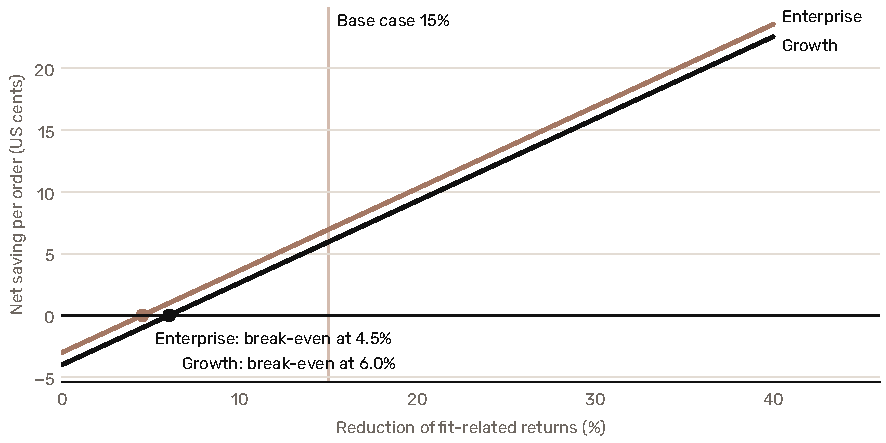
\includegraphics[width=\textwidth]{figures/f6-retailer-economics.pdf}
\caption{Retailer's economics against the achieved reduction $\rho$ (derived)}\label{fig:f6}
\end{figure}

\ctchapterend
